\icode{E-MC-SI-L3-261026-001}
如图所示，相同的小球\(A\)、\(B\)静止在水平面上，用长为\(L\)的细线连接，细线刚好伸直，\(O\)为细线的中点，用竖直向上的力作用在\(O\)点，使\(O\)点竖直向上运动，当\(A\)、\(B\)间的距离变为\(\frac{L}{2}\)时，\(O\)点的速度大小为\(v\)，则此时\(A\)球的速度大小为\paren[]

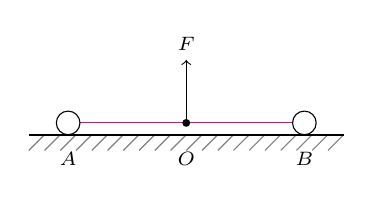
\begin{tikzpicture}[font=\scriptsize]
	\draw[magenta] (-1.5,.15)--(1.5,.15);
	\draw[->] (0,.15)--++(0,.8)node[above]{\(F\)};
	\fill (0,.15) circle(.05);
	\draw[fill=white] (-1.5,.15) circle(.15) (1.5,.15) circle(.15);
	\foreach \x in {-2,-1.8,...,1.8}
		\draw[gray] (\x,-.2)--++(.2,.2);
	\draw[thick] (-2,0)--(2,0);
	\node at(-1.5,-.1)[below]{\(A\)};
	\node at(0,-.1)[below]{\(O\)};
	\node at(1.5,-.1)[below]{\(B\)};
\end{tikzpicture}
\begin{choices}
	\item\(\sqrt{3}v\)
	\item\(\dfrac{\sqrt{3}}{2}v\)
	\item\(\dfrac{\sqrt{3}}{3}v\)
	\item\(\dfrac{2 \sqrt{3}}{3}v\)
\end{choices}
\begin{answer}
    
\end{answer}